\documentclass[aspectratio=169,compress]{beamer}
\usepackage[T1]{fontenc}
\usepackage{lmodern}
\usepackage{graphicx}
\usepackage{xcolor}
\usepackage{textcomp}
\usepackage{booktabs}
\usepackage{array}
\usepackage{tikz}
\usetikzlibrary{arrows.meta}

% Match the established FRIDA slide style.
\definecolor{NordBody}{HTML}{4C566A}
\definecolor{NordBlue}{HTML}{5E81AC}
\definecolor{NordPanel}{HTML}{ECEFF4}

\setbeamertemplate{footline}{%
  \hspace{1em}%
  \usebeamercolor[fg]{page number in head/foot}%
  \usebeamerfont{page number in head/foot}%
  \insertframenumber\,/\,\inserttotalframenumber%
  \vskip2pt%
}
\beamertemplatenavigationsymbolsempty
\setbeamerfont{frametitle}{size=\large}
\setbeamercolor{normal text}{fg=NordBody}
\setbeamercolor{title}{fg=NordBlue}
\setbeamercolor{frametitle}{fg=NordBlue}
\setbeamercolor{structure}{fg=NordBlue}
\setbeamercolor{itemize item}{fg=NordBlue}
\setbeamercolor{block title}{fg=NordBlue,bg=NordPanel}
\setbeamercolor{block body}{fg=NordBody,bg=NordPanel!55}
\hypersetup{colorlinks=true,allcolors=NordBlue}

\newcommand{\pin}[1]{\texttt{\detokenize{#1}}}
\newcommand{\rail}[1]{\texttt{\detokenize{#1}}}

\title{FRIDA ADC Integration Guide}
\author{Kennedy Caisley}
\institute{University of Bonn}
\date{18 August 2026}

\begin{document}

\section[Interface]{Interface}
\begin{frame}
  \frametitle{ADC pinout}
  \begin{columns}[T,onlytextwidth]
    \begin{column}{0.405\textwidth}
      \centering
      \vspace{0.25em}
      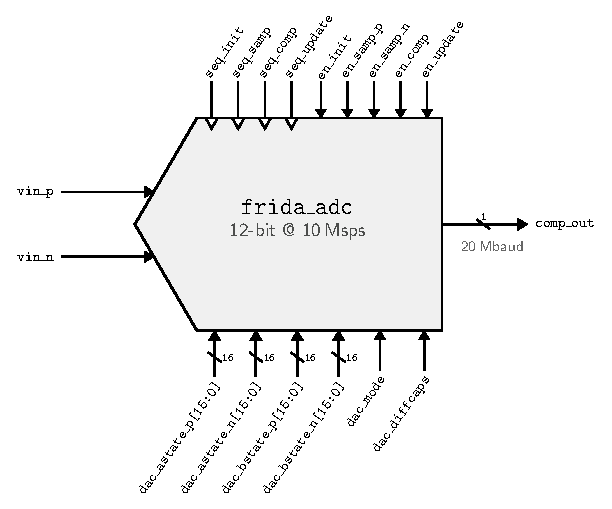
\includegraphics[width=\linewidth,height=0.73\textheight,keepaspectratio]{../images/adc_symbol.pdf}
    \end{column}
    \begin{column}{0.575\textwidth}
      \fontsize{6.8}{7.6}\selectfont
      \setlength{\tabcolsep}{3pt}
      \renewcommand{\arraystretch}{1.18}
      \begin{tabular}{@{}>{\raggedright\arraybackslash}p{0.28\linewidth}
                          >{\raggedright\arraybackslash}p{0.42\linewidth}
                          >{\raggedright\arraybackslash}p{0.24\linewidth}@{}}
        \toprule
        \textbf{Pin group} & \textbf{Purpose} & \textbf{Default / operating value} \\
        \midrule
        \pin{vin_p}, \pin{vin_n} & Differential analog input & $V_\mathrm{CM}=0.615$ V; best at 0.6--0.7 V \\
        \pin{seq_init} & Load the A state and reset the SAR trial & 0 when idle \\
        \pin{seq_samp} & Drive the differential sampling phase & 0 when idle \\
        \pin{seq_comp} & Clock comparator evaluations & 0 when idle \\
        \pin{seq_update} & Commit each SAR decision & 0 when idle \\
        \pin{en_init}, \pin{en_samp_p/n}, \pin{en_comp}, \pin{en_update} & Gate the corresponding internal clocks & all 1 \\
        \pin{dac_mode}, \pin{dac_diffcaps} & Select comparator-driven SAR updates and differential-cap control & 1, 1 \\
        \pin{dac_astate_p/n}\newline\pin{[15:0]} & Initial P/N CDAC state & \pin{16'h5555} (0101\ldots) \\
        \pin{dac_bstate_p/n}\newline\pin{[15:0]} & Alternate/test P/N CDAC state & \pin{16'h0000} \\
        \pin{comp_out} & Single-ended comparator readout & output \\
        \bottomrule
      \end{tabular}
    \end{column}
  \end{columns}
\end{frame}

\section[Power]{Power}
\begin{frame}
  \frametitle{Power rails}
  \vspace{0.35em}
  \centering
  \renewcommand{\arraystretch}{1.15}
  \begin{tabular}{@{}>{\raggedright\arraybackslash}p{0.20\linewidth}
                      >{\raggedright\arraybackslash}p{0.47\linewidth}
                      >{\raggedleft\arraybackslash}p{0.20\linewidth}@{}}
    \toprule
    \textbf{Power pins} & \textbf{What the domain supplies} & \textbf{Power at 10 MS/s} \\
    \midrule
    \rail{vdd_a / vss_a} & Comparator, sampling switches, and local comparator-clock inversion & \textbf{3 \textmu W} \\
    \rail{vdd_d / vss_d} & SAR state, clock gating, sequencer distribution, and sampling-clock drivers & \textbf{451--457 \textmu W} \\
    \rail{vdd_dac / vss_dac} & CDAC bottom-plate drivers and reference switching & \textbf{34 \textmu W} \\
    \midrule
    \textbf{Measured total} & Whole-chip reading with one ADC active & \textbf{488--494 \textmu W} \\
    \bottomrule
  \end{tabular}

  \vfill
  {\scriptsize (Measured on ADC00 and ADC01 at 1.2 V and 10 MS/s.)}
\end{frame}

\section[Layout]{Layout}
\begin{frame}
  \frametitle{Layout view}
  \centering
  \begin{tikzpicture}
    \node[inner sep=0pt] (adc) {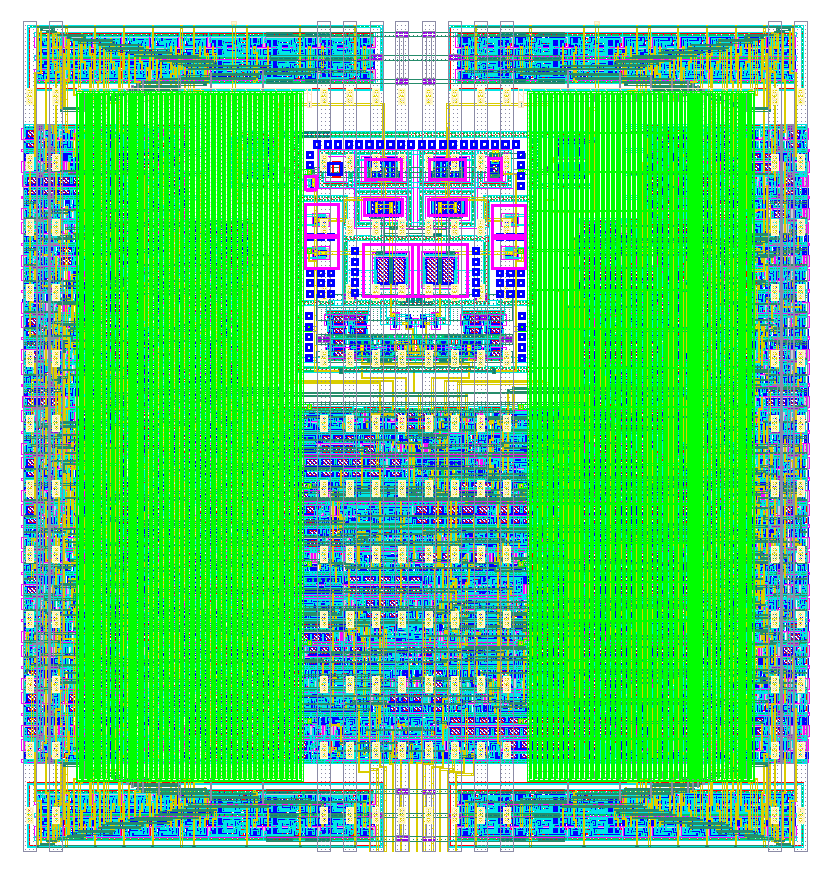
\includegraphics[height=0.72\textheight,keepaspectratio]{../images/frida_adc.png}};
    \draw[{Stealth[length=2mm]}-{Stealth[length=2mm]}, line width=0.7pt, draw=NordBlue]
      ([yshift=-0.18cm]adc.south west) -- node[below,font=\scriptsize,text=NordBody]{60.5 \textmu m} ([yshift=-0.18cm]adc.south east);
    \draw[{Stealth[length=2mm]}-{Stealth[length=2mm]}, line width=0.7pt, draw=NordBlue]
      ([xshift=-0.18cm]adc.south west) -- node[left,font=\scriptsize,text=NordBody]{63.5 \textmu m} ([xshift=-0.18cm]adc.north west);
  \end{tikzpicture}
\end{frame}

\section[Sequence]{Sequence}
\begin{frame}
  \frametitle{Control sequence}
  \centering
  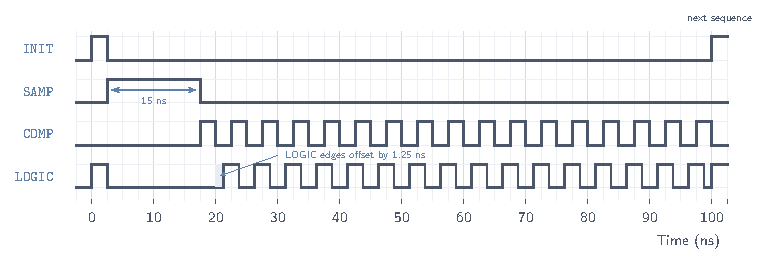
\includegraphics[width=0.985\linewidth,height=0.43\textheight,keepaspectratio]{../images/adc_sequencer_timing.pdf}

  \vspace{0.2em}
  \fontsize{7.2}{8.0}\selectfont
  \renewcommand{\arraystretch}{1.08}
  \begin{tabular}{@{}>{\raggedright\arraybackslash}p{0.13\linewidth}
                      >{\raggedright\arraybackslash}p{0.20\linewidth}
                      >{\raggedright\arraybackslash}p{0.52\linewidth}@{}}
    \toprule
    \textbf{Track} & \textbf{ADC pin} & \textbf{Required action} \\
    \midrule
    INIT & \pin{seq_init} & Pulse INIT and LOGIC together for one 2.5 ns window. \\
    SAMP & \pin{seq_samp} & Hold high for 15 ns to acquire both differential inputs. \\
    COMP & \pin{seq_comp} & Apply seventeen 2.5 ns high windows on a 5 ns period. \\
    LOGIC & \pin{seq_update} & Pulse once with INIT, then apply sixteen delayed 2.5 ns update windows. \\
    \bottomrule
  \end{tabular}
\end{frame}

\end{document}
